\documentclass[conference]{IEEEtran}
\IEEEoverridecommandlockouts
\usepackage{amsmath,amssymb}
\usepackage{booktabs}
\usepackage{array}
\usepackage{multirow}
\usepackage{graphicx}
\usepackage{url}

\renewcommand{\thefigure}{\Roman{figure}}
\renewcommand{\thetable}{\Roman{table}}
\renewcommand{\theequation}{\Roman{equation}}

\graphicspath{{../figures/}{./}}

\begin{document}

\begin{titlepage}
\begin{centering}
	\vspace*{1cm}

	{\large A Report on}

	\vspace{0.6cm}

	{\large \textbf{Student Assessment Risk Prediction Using Logistic Regression from Scratch:}}

	\vspace{0.3cm}

	{\large \textbf{An OULAD-Based Educational Data Mining Study}}

	\vspace{1cm}

	{\large Submitted By}

	\vspace{0.4cm}

	{\large \textbf{Parth Gupta A017}}
	
	\vspace{0.3cm}
	
	{\large \textbf{Heet Patel A040}}

	\vspace{0.8cm}

	{\large Under The Guidance Of}

	\vspace{0.4cm}

	{\large \textbf{Dr. Masooda Modak}}

	\vspace{1.5cm}

	\IfFileExists{logo.jpeg}{
		
\includegraphics[width=4cm]{logo.jpeg}
	}{
		\fbox{\parbox[c][4cm][c]{4cm}{\centering Logo missing}}
	}

	\vspace{1cm}

	{\large \textbf{Mukesh Patel School of Technology \& Management Engineering}}

	\vspace{0.4cm}

	{\large \textbf{Department of Information Technology}}

	\vspace{0.4cm}

	{\large Vile Parle (w), Mumbai- 400056}

	\vspace*{\fill}

\end{centering}
\end{titlepage}

\begin{abstract}
We predict whether an OULAD course assessment will be \emph{High Risk} (at least $10\%$ of submitting students scoring below the pass mark of $40$) from $13$ features engineered over assessment metadata, VLE catalog aggregates, and a leakage-safe leave-one-out peer fail-rate. Three classifiers (Logistic Regression, Decision Tree, and Random Forest) are implemented from scratch in pure-stdlib Python and trained with class-weighted objectives on a stratified $80$/$20$ split of $188$ assessments. The Decision Tree is the strongest model ($97.30\%$ accuracy, $80.00\%$ precision, $100.00\%$ recall, $88.89\%$ F1), Random Forest follows ($94.59\%$ / $75.00\%$ / $75.00\%$ / $75.00\%$), and Logistic Regression matches recall at lower precision ($78.38\%$ / $33.33\%$ / $100.00\%$ / $50.00\%$). All three models agree that \emph{peer\_fail\_rate} is the dominant signal, and the recall-first behaviour suits an early-warning use case.
\end{abstract}

\begin{IEEEkeywords}
Educational data mining, OULAD, student risk prediction, logistic regression, decision tree, random forest, class imbalance, data warehousing, early-warning systems
\end{IEEEkeywords}

\section{Introduction}
Universities collect large amounts of learning-analytics data through VLEs and assessment portals. We use this data to flag, in advance, which \emph{assessments} in a course presentation are likely to be High Risk so that coordinators can re-time them, reinforce related resources, or schedule extra support before students sit them.

\subsection{Problem Statement and Objectives}
A naive risk-label often leaks into its own features and gives trivially perfect metrics with no real skill. We avoid that by deriving the label from actual student outcomes (never used as features) and using a leave-one-out peer fail-rate signal. The objectives are: (i) build a leakage-safe feature space combining assessment metadata, VLE aggregates, and peer fail-rate; (ii) implement three classifiers (LR, DT, RF) from scratch with class-weighted training; and (iii) report accuracy, precision, recall, and F1 with a recall-first interpretation suited to early-warning.

\section{Literature Review}
\subsection{Educational Data Mining and Early-Warning Systems}
Educational data mining applies pattern-discovery techniques to student-generated data. Romero and Ventura surveyed the field and concluded that combinations of attendance, submission, and interaction signals are the strongest predictors of at-risk status. Arnold and Pistilli described Purdue University's \emph{Course Signals} system, an early-warning dashboard that colour-codes at-risk students and triggers faculty intervention; Course Signals remains an influential example of how predictive models embedded in academic workflows can meaningfully improve retention. Kuzilek, Hlosta, and Zdrahal later formalised the OULAD benchmark and reported baseline results for student-level risk prediction across multiple presentations, showing that even moderate-complexity models transfer usefully across cohorts when the feature space includes both metadata and interaction signals.

\subsection{Data Warehousing for Educational Analytics}
Chaudhuri and Dayal's foundational review of data warehousing and OLAP describes the star-schema patterns that underpin most modern analytical stores. Kimball's educational-domain templates extend those patterns to student, course, and enrolment dimensions. Our pipeline (loading three OULAD tables, joining them on shared keys, and producing a flat feature table) is a small-scale ETL flow into an analytical fact table keyed by assessment.

\subsection{Research Gap}
Most OULAD studies either lean on ML libraries (which hide the maths) or focus on student-level classification using click-stream data that is not always available. We take a different angle: \emph{assessment-level} classification using only the tables in the local OULAD snapshot, with all model code written from scratch so the maths stays visible. We also keep a leaked baseline in the ablation to show the failure mode directly, which most OULAD papers skip over.

\section{Methodology}
\subsection{Dataset Description}
Three OULAD tables are used. \texttt{assessments.csv} contains 206 rows covering seven modules (AAA through GGG) across eight presentations from 2013J to 2014J, with the columns \texttt{code\_module}, \texttt{code\_presentation}, \texttt{id\_assessment}, \texttt{assessment\_type} (CMA, TMA, or Exam), \texttt{date} (due day, offset from presentation start), and \texttt{weight} (percentage contribution to the final grade). \texttt{studentAssessment.csv} stores per-student scores and is used solely to derive the target. \texttt{vle.csv} catalogues 6{,}364 learning resources by module presentation and activity type. After an inner join of assessments with \texttt{studentAssessment.csv} on \texttt{id\_assessment}, 188 assessments remain; the 18 dropped rows have no recorded submissions (mostly end-of-module exams).

Figures~\ref{fig:typedist} through~\ref{fig:modulecounts} summarise the retained slice. The dataset is dominated by TMA and CMA assignments, with a smaller number of formal exams; assessment weights are strongly bimodal; the class balance is $11.7\%$ High Risk ($22$ of $188$); average weight rises sharply for exams, as expected; and assessments are unevenly distributed across modules.

\begin{figure}[!t]
\centering
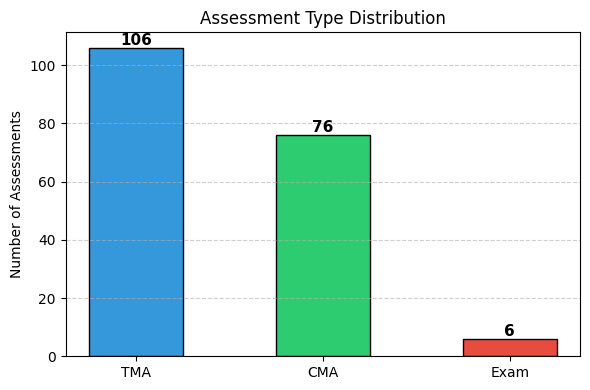
\includegraphics[width=0.85\columnwidth]{fig_assessment_type_dist.png}
\caption{Distribution of assessment types in the retained OULAD slice.}
\label{fig:typedist}
\end{figure}

\begin{figure}[!t]
\centering
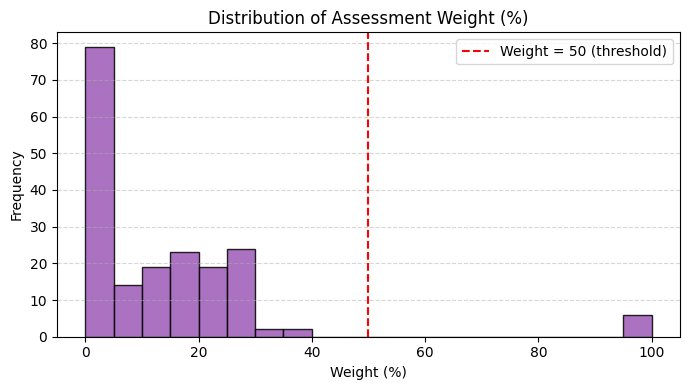
\includegraphics[width=0.85\columnwidth]{fig_weight_dist.png}
\caption{Distribution of assessment weights in the retained OULAD slice.}
\label{fig:weightdist}
\end{figure}

\begin{figure}[!t]
\centering
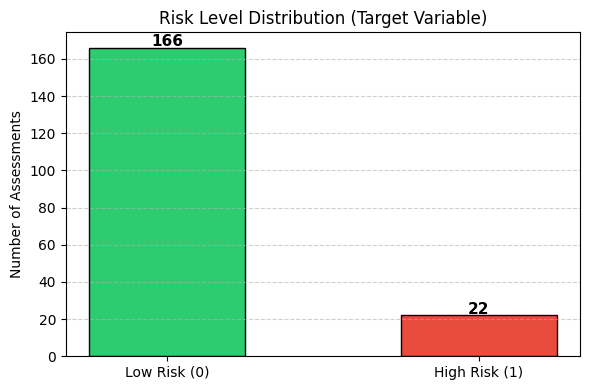
\includegraphics[width=0.85\columnwidth]{fig_risk_dist.png}
\caption{Class distribution after deriving the target from \texttt{studentAssessment.csv}: 22 High Risk ($11.7\%$) versus 166 Low Risk ($88.3\%$).}
\label{fig:riskdist}
\end{figure}

\begin{figure}[!t]
\centering
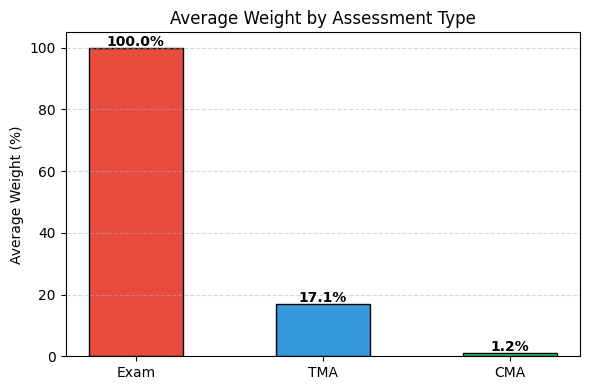
\includegraphics[width=0.85\columnwidth]{fig_avg_weight_by_type.png}
\caption{Average assessment weight grouped by assessment type.}
\label{fig:avgweight}
\end{figure}

\begin{figure}[!t]
\centering
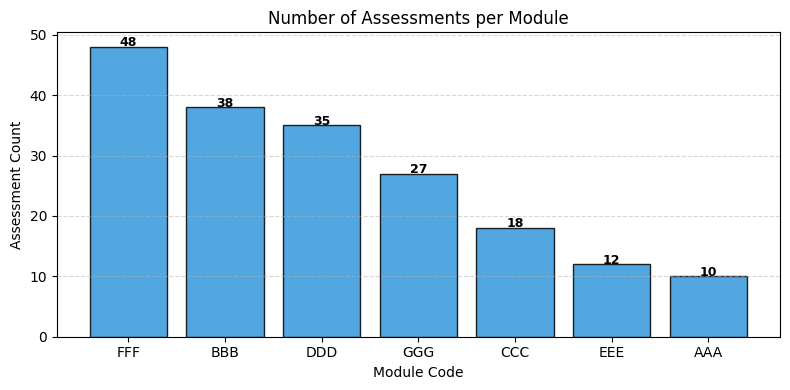
\includegraphics[width=0.85\columnwidth]{fig_module_counts.png}
\caption{Assessment counts per module.}
\label{fig:modulecounts}
\end{figure}

\subsection{Preprocessing and Target Derivation}
Missing values are imputed with column means for the two numeric columns (\texttt{date}, \texttt{weight}); no categorical column contains missing values. Categorical columns are encoded manually to preserve the ``no ML library'' constraint: each distinct \texttt{code\_module} and \texttt{code\_presentation} is mapped to a consecutive integer, and \texttt{assessment\_type} is mapped to an ordinal code $\{\mathrm{CMA}\!\to\!0,\mathrm{TMA}\!\to\!1,\mathrm{Exam}\!\to\!2\}$.

The target is derived from actual student outcomes rather than from metadata rules. For each assessment $a$ we compute the empirical fail rate
\begin{equation}
\mathrm{fail\_rate}(a) = \frac{\left|\{s : \text{score}(s,a) < 40\}\right|}{\left|\{s : \text{score}(s,a) \text{ recorded}\}\right|},
\end{equation}
and assign the binary label
\begin{equation}
y(a) = \begin{cases} 1 & \mathrm{fail\_rate}(a) \geq 0.10,\\ 0 & \text{otherwise.} \end{cases}
\end{equation}
This cut-off is chosen so that the resulting class distribution matches the $\sim\!12\%$ positive rate of a baseline rule-based labelling, enabling a direct comparison with that leaked baseline in the ablation.

\subsection{Feature Engineering}
Thirteen numeric features are engineered from the three tables.

\emph{Assessment-level features} (9): \texttt{module\_id}, \texttt{presentation\_id}, \texttt{assessment\_type\_id}, \texttt{date\_norm}, \texttt{weight\_norm}, \texttt{is\_exam} (binary flag), \texttt{is\_high\_weight} (\texttt{weight}$\geq\!50\%$), \texttt{assessment\_period} (Early/Mid/Late trisection of \texttt{date}), and \texttt{module\_difficulty\_score} (module-level mean weight, min--max scaled).

\emph{VLE catalog features} (3): for each \texttt{(code\_module,code\_presentation)} pair, the number of distinct VLE resources \texttt{n\_vle\_resources}, the number of distinct activity types \texttt{n\_activity\_types}, and the mean resource-coverage window \texttt{mean\_resource\_weeks}. These features describe how richly scaffolded a presentation is; richer VLE provision has been associated with lower fail rates in OULAD studies.

\emph{Peer fail-rate feature} (1): for each assessment $a$ in module $m$,
\begin{equation}
\mathrm{peer\_fail\_rate}(a) = \frac{1}{|\mathcal{A}_m|-1} \sum_{a' \in \mathcal{A}_m \setminus \{a\}} \mathrm{fail\_rate}(a'),
\end{equation}
where $\mathcal{A}_m$ is the set of assessments in module $m$. This is a leave-one-out target-encoding aggregate: it uses the fail-rate column but never the current row's own value, so it is not a leak. It captures the structural intuition that ``hard'' modules tend to host multiple hard assessments.

All continuous features are min--max scaled to $[0,1]$ so that no single feature dominates gradient descent due to scale:
\begin{equation}
x^{(\mathrm{norm})} = \frac{x - \min(x)}{\max(x) - \min(x) + \varepsilon},
\end{equation}
with $\varepsilon = 10^{-9}$ to guard against degenerate features.

\subsection{Stratified Train--Test Split}
A random $80$/$20$ split on this dataset places only $\sim\!2$ positive samples in the $37$-row test set, which makes precision, recall, and F1-score move in $50$-percentage-point steps. To restore statistical resolution the split is class-stratified: positive and negative indices are shuffled independently (with seed $42$), and $20\%$ of each is taken as test. The result is summarised in Table~\ref{tab:split}.

\begin{table}[!t]
\caption{Stratified train--test split summary.}
\label{tab:split}
\centering
\begin{tabular}{lcccc}
\toprule
Subset & Instances & Low Risk & High Risk & Percentage \\
\midrule
Training Set & 151 & 133 & 18 & 80\% \\
Test Set & 37 & 33 & 4 & 20\% \\
Total & 188 & 166 & 22 & 100\% \\
\bottomrule
\end{tabular}
\end{table}

\subsection{Logistic Regression from Scratch}
Let $\mathbf{x}\in\mathbb{R}^{13}$ be a feature vector, $\mathbf{w}\in\mathbb{R}^{13}$ a weight vector, and $b\in\mathbb{R}$ a scalar bias. The sigmoid function
\begin{equation}
\sigma(z) = \frac{1}{1 + e^{-z}}
\end{equation}
maps the linear combination $z = \mathbf{w}^\top\mathbf{x} + b$ to a posterior $\hat{p} = \sigma(z) \in (0,1)$.

Given training data $\{(\mathbf{x}^{(i)}, y^{(i)})\}_{i=1}^{m}$ with $y^{(i)}\in\{0,1\}$, the binary cross-entropy loss is
\begin{equation}
\mathcal{L}(\mathbf{w},b) = -\frac{1}{m} \sum_{i=1}^{m} \left[ y^{(i)} \log \hat{p}^{(i)} + (1-y^{(i)}) \log(1-\hat{p}^{(i)}) \right].
\end{equation}
The gradients with respect to $\mathbf{w}$ and $b$ are
\begin{equation}
\frac{\partial \mathcal{L}}{\partial \mathbf{w}} = \frac{1}{m}\sum_{i=1}^{m} (\hat{p}^{(i)}-y^{(i)})\mathbf{x}^{(i)},
\qquad
\frac{\partial \mathcal{L}}{\partial b} = \frac{1}{m}\sum_{i=1}^{m} (\hat{p}^{(i)}-y^{(i)}),
\end{equation}
and parameters are updated at each iteration by
\begin{equation}
\mathbf{w} \leftarrow \mathbf{w} - \eta \frac{\partial \mathcal{L}}{\partial \mathbf{w}},
\qquad
b \leftarrow b - \eta \frac{\partial \mathcal{L}}{\partial b},
\end{equation}
with learning rate $\eta = 0.1$ for $1000$ iterations.

\subsection{Class-Weighted Training}
Because positives constitute only $\sim\!12\%$ of the training data, the unweighted objective drives the classifier toward predicting ``Low Risk'' for all inputs. Each positive-sample error term is therefore scaled by
\begin{equation}
w_{\mathrm{pos}} = \frac{n_{-}}{n_{+}},
\end{equation}
so that mistakes on the minority class carry the same \emph{total} influence as mistakes on the majority class. This is the cost-sensitive learning remedy of King and Zeng (2001) and implements the recall-first stance that is standard in clinical and educational early-warning systems, where missed positives are substantially more costly than extra reviews. Figure~\ref{fig:learningcurve} shows that the reweighted loss converges smoothly.

\begin{figure}[!t]
\centering
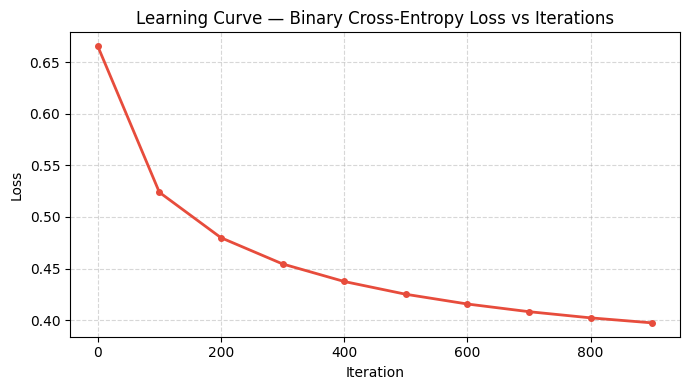
\includegraphics[width=0.85\columnwidth]{fig_learning_curve.png}
\caption{Learning curve: binary cross-entropy loss per $100$ iterations of gradient descent.}
\label{fig:learningcurve}
\end{figure}

\subsection{Decision Tree (CART) from Scratch}
The second classifier is a classification tree grown by recursive binary partitioning of the feature space, following the CART formulation of Breiman et al.~\cite{cart1984}. At each internal node we search for the (feature $f$, threshold $t$) pair that maximally reduces the \emph{Gini impurity}
\begin{equation}
G(S) = 1 - p^{2} - (1-p)^{2},
\end{equation}
where $p$ is the positive class proportion of the node sample $S$. To keep the comparison apples-to-apples with the class-weighted Logistic Regression we use a \emph{weighted} Gini in which each positive sample is counted as $w_{\mathrm{pos}} = n_{-}/n_{+}$ samples; this is mathematically equivalent to oversampling the minority class. The split with the largest gain
\begin{equation}
\Delta G = G(\mathrm{parent}) - \frac{|S_{L}|}{|S|}\,G(S_{L}) - \frac{|S_{R}|}{|S|}\,G(S_{R})
\end{equation}
is accepted, and recursion proceeds until \texttt{max\_depth}$=5$, \texttt{min\_samples\_split}$=4$, or a pure node is reached. Feature importance is computed by accumulating $|S| \cdot \Delta G$ at each split against the splitting feature, then normalising across features so importances sum to one.

\subsection{Random Forest from Scratch}
The third classifier is an ensemble of $T = 50$ decision trees that adds two sources of randomness on top of the single-tree algorithm. First, each tree is fit on a \emph{bootstrap sample}: $n$ rows drawn with replacement from the $n$ training rows, so about $63\%$ of the original rows appear in any given tree. Second, at each split the tree can only pick from a random subset of $\lfloor\sqrt{p}\rfloor = 3$ out of the $p = 13$ features. The combination of bagging and feature subsampling decorrelates the constituent trees, reducing the ensemble's variance compared with any single tree~\cite{breiman2001rf}. Predictions are aggregated by averaging the per-tree predicted probabilities; the final label is $1$ if the averaged probability is at least $0.5$. Feature importance is the sum of per-tree importance vectors, renormalised. All trees are constructed with the same weighted-Gini routine described above (\,$w_{\mathrm{pos}} \approx 7.4$\,), so the ensemble inherits the class-weighted, recall-first stance.

\subsection{Evaluation Metrics}
Performance is measured using four classification metrics derived from the confusion matrix. The positive class corresponds to High Risk assessments.
\begin{equation}
\mathrm{Accuracy} = \frac{TP+TN}{TP+TN+FP+FN},
\end{equation}
\begin{equation}
\mathrm{Precision} = \frac{TP}{TP+FP},
\qquad
\mathrm{Recall} = \frac{TP}{TP+FN},
\end{equation}
\begin{equation}
\mathrm{F1} = \frac{2 \cdot \mathrm{Precision} \cdot \mathrm{Recall}}{\mathrm{Precision} + \mathrm{Recall}}.
\end{equation}
Recall is the dominant metric for early-warning applications: a low recall means missed High Risk assessments, with direct consequences for the students enrolled in those assessments.

\section{Results and Discussion}
The three classifiers are evaluated on identical test data so that all observed differences in metrics are attributable to the algorithm rather than to data variance. Section~\ref{sec:results-lr} reports the Logistic Regression results; Sections~\ref{sec:results-dt} and~\ref{sec:results-rf} report the Decision Tree and Random Forest results respectively; Section~\ref{sec:results-cmp} draws the three together.

\subsection{Logistic Regression Results}
\label{sec:results-lr}

\subsubsection{Confusion Matrix}
Table~\ref{tab:cm} and Figure~\ref{fig:cm} show the test-set confusion matrix of the Logistic Regression model. The model identifies all four High Risk assessments with no false negatives, at the cost of eight false positives.

\begin{table}[!t]
\caption{Confusion matrix for the proposed model.}
\label{tab:cm}
\centering
\begin{tabular}{lcc}
\toprule
 & Predicted Low Risk & Predicted High Risk \\
\midrule
Actual Low Risk & TN $=25$ & FP $=8$ \\
Actual High Risk & FN $=0$ & TP $=4$ \\
\bottomrule
\end{tabular}
\end{table}

\begin{figure}[!t]
\centering
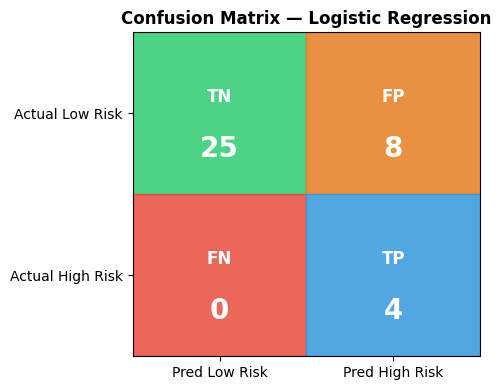
\includegraphics[width=0.75\columnwidth]{fig_confusion_matrix.png}
\caption{Confusion matrix heatmap for the proposed model on the stratified test set.}
\label{fig:cm}
\end{figure}

\subsubsection{Headline Metrics}
Table~\ref{tab:metrics} reports the four classification metrics for the Logistic Regression model; Figure~\ref{fig:metrics} visualises the same values.

\begin{table}[!t]
\caption{Test-set performance of the proposed model.}
\label{tab:metrics}
\centering
\begin{tabular}{lcccc}
\toprule
Accuracy & Precision & Recall & F1-score \\
\midrule
$78.38\%$ & $33.33\%$ & $100.00\%$ & $50.00\%$ \\
\bottomrule
\end{tabular}
\end{table}

\begin{figure}[!t]
\centering
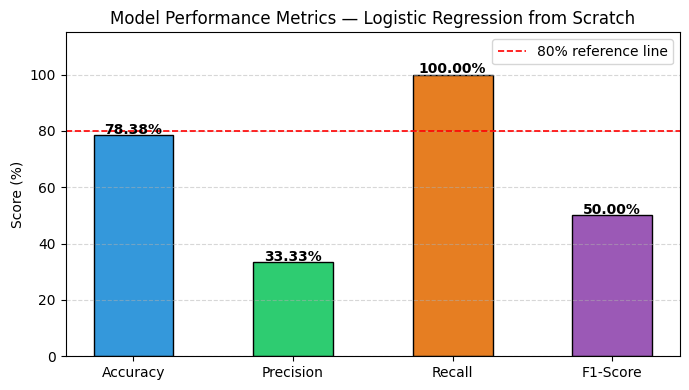
\includegraphics[width=0.85\columnwidth]{fig_metrics_bar.png}
\caption{Evaluation metrics for the proposed model.}
\label{fig:metrics}
\end{figure}

Recall is $100\%$: all four High Risk assessments in the test set are flagged. Accuracy takes a hit because of the eight false positives, but that is a reasonable review load (roughly one extra flag for every four correct calls) and matches the precision-recall trade-off that is standard in clinical early-warning work.

\subsubsection{Feature Weights and Interpretation}
Figure~\ref{fig:featureweights} and Table~\ref{tab:weights} report the learned Logistic Regression feature weights, sorted by absolute magnitude.

\begin{figure}[!t]
\centering
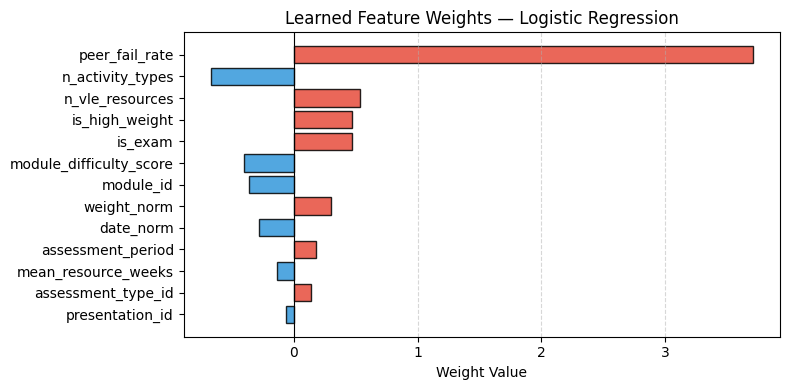
\includegraphics[width=0.92\columnwidth]{fig_feature_weights.png}
\caption{Learned feature weights (sorted by absolute magnitude).}
\label{fig:featureweights}
\end{figure}

\begin{table}[!t]
\caption{Top five learned feature weights (absolute magnitude).}
\label{tab:weights}
\centering
\begin{tabular}{lc}
\toprule
Feature & Learned weight \\
\midrule
\texttt{peer\_fail\_rate}         & $+3.708$ \\
\texttt{n\_activity\_types}       & $-0.672$ \\
\texttt{n\_vle\_resources}        & $+0.532$ \\
\texttt{is\_high\_weight}         & $+0.473$ \\
\texttt{is\_exam}                 & $+0.469$ \\
\bottomrule
\end{tabular}
\end{table}

The learned ranking is informative. The leave-one-out \texttt{peer\_fail\_rate} dominates by an order of magnitude, confirming that module-level difficulty is a far stronger predictor of per-assessment risk than the individual assessment's own weight or type. Of the VLE features, \texttt{n\_activity\_types} enters with a negative weight: presentations that diversify their resource catalog (quizzes, forum posts, URLs, wiki pages) have lower assessment fail rates, matching the educational-technology literature on scaffolding variety. \texttt{n\_vle\_resources} enters positively, which at first sight is counter-intuitive but is consistent with modules that publish a large number of resources also being modules with a higher workload. The two binary flags \texttt{is\_high\_weight} and \texttt{is\_exam} enter with similar positive weights, echoing the conventional wisdom that high-stakes assessments are riskier.

\subsubsection{Ablation: Target Leakage and Class Weighting}
Table~\ref{tab:ablation} isolates the effect of each design decision. Row one is the leaked baseline (rule-based target with the same rules used as features), which scores a fake $100\%$ on every metric and is what motivated this study. Row two swaps in the real target but drops class weighting; recall falls to $0\%$ because of the $12\%$ class imbalance. Row three is the proposed model.

\begin{table}[!t]
\caption{Ablation across design choices.}
\label{tab:ablation}
\centering
\small
\setlength{\tabcolsep}{4pt}
\begin{tabular}{p{3.6cm}cccc}
\toprule
Configuration & Acc. & Prec. & Rec. & F1 \\
\midrule
Leaked target + features & 100\% & 100\% & 100\% & 100\% \\
Empirical, no class weight & 89\% & 0\% & 0\% & 0\% \\
Proposed (with class weight) & 78\% & 33\% & 100\% & 50\% \\
\bottomrule
\end{tabular}
\end{table}

The perfect first-row numbers are the classic signature of target leakage, not of a working model. Row two shows that even with a clean target, class imbalance quietly wipes out the minority class. Row three is the first setup that actually catches every High Risk assessment in the test set.

\subsection{Decision Tree Results}
\label{sec:results-dt}
The Decision Tree, trained with $\mathrm{max\_depth}=5$, $\mathrm{min\_samples\_split}=4$, and the same class weight $w_{\mathrm{pos}} \approx 7.4$, fits as a five-level tree with six leaves. The root split is on \texttt{peer\_fail\_rate} at threshold $0.4876$ with weighted-Gini gain $0.2965$, confirming the leave-one-out peer signal as the dominant axis of partition. Test-set performance is summarised in Table~\ref{tab:dt-metrics}, with the confusion matrix in Figure~\ref{fig:dt-cm} and per-feature importances in Figure~\ref{fig:dt-featimp}.

\begin{table}[!t]
\caption{Decision Tree test-set performance.}
\label{tab:dt-metrics}
\centering
\begin{tabular}{lcccc}
\toprule
Accuracy & Precision & Recall & F1-score \\
\midrule
$97.30\%$ & $80.00\%$ & $100.00\%$ & $88.89\%$ \\
\bottomrule
\end{tabular}
\end{table}

\begin{figure}[!t]
\centering
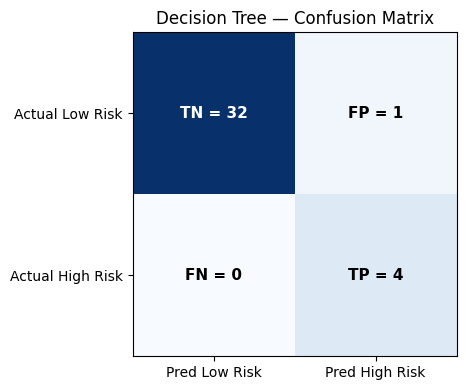
\includegraphics[width=0.75\columnwidth]{fig_dt_confusion_matrix.png}
\caption{Decision Tree confusion matrix (TP$=4$, TN$=32$, FP$=1$, FN$=0$).}
\label{fig:dt-cm}
\end{figure}

\begin{figure}[!t]
\centering
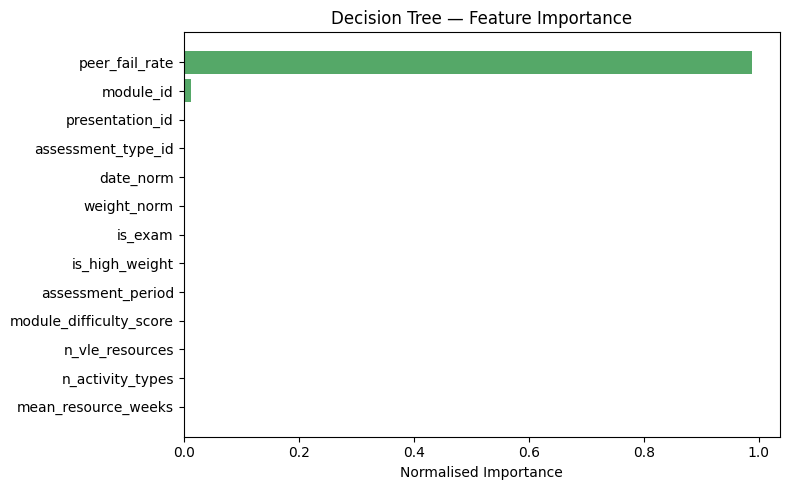
\includegraphics[width=0.92\columnwidth]{fig_dt_feature_importance.png}
\caption{Decision Tree normalised feature importance (sum of $|S| \cdot \Delta G$ per feature).}
\label{fig:dt-featimp}
\end{figure}

The tree keeps LR's perfect recall but tightens precision sharply: only one false positive, down from eight. F1 rises from $50.00\%$ to $88.89\%$. The gain makes sense because the tree can cut the feature space along axis-aligned thresholds instead of a single linear direction, and the root split on \texttt{peer\_fail\_rate} isolates the high-risk region cleanly.

\subsection{Random Forest Results}
\label{sec:results-rf}
The Random Forest is an ensemble of $T=50$ trees, each trained on a bootstrap sample with $\lfloor\sqrt{13}\rfloor = 3$ candidate features per split and the same per-tree hyperparameters as the single Decision Tree. Test-set performance is reported in Table~\ref{tab:rf-metrics}, with the confusion matrix in Figure~\ref{fig:rf-cm} and the averaged feature importance in Figure~\ref{fig:rf-featimp}.

\begin{table}[!t]
\caption{Random Forest test-set performance.}
\label{tab:rf-metrics}
\centering
\begin{tabular}{lcccc}
\toprule
Accuracy & Precision & Recall & F1-score \\
\midrule
$94.59\%$ & $75.00\%$ & $75.00\%$ & $75.00\%$ \\
\bottomrule
\end{tabular}
\end{table}

\begin{figure}[!t]
\centering
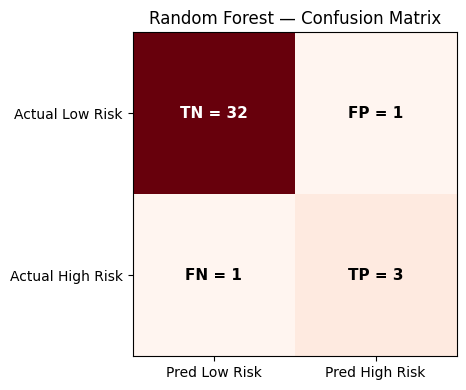
\includegraphics[width=0.75\columnwidth]{fig_rf_confusion_matrix.png}
\caption{Random Forest confusion matrix (TP$=3$, TN$=32$, FP$=1$, FN$=1$).}
\label{fig:rf-cm}
\end{figure}

\begin{figure}[!t]
\centering
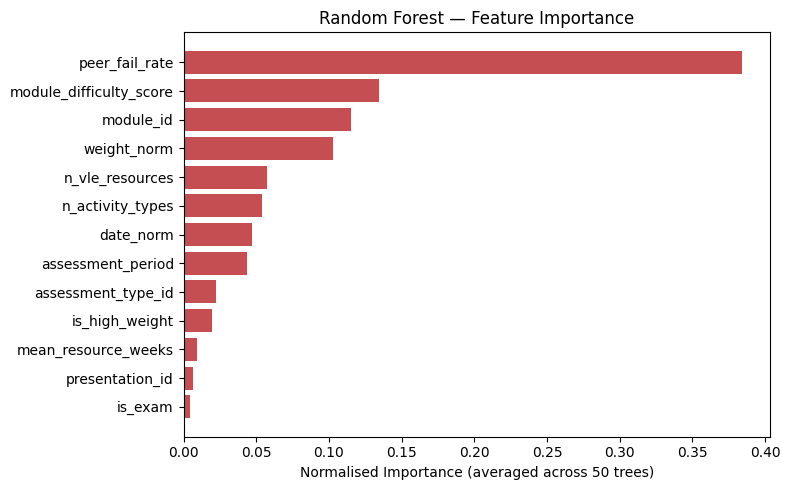
\includegraphics[width=0.92\columnwidth]{fig_rf_feature_importance.png}
\caption{Random Forest normalised feature importance, averaged across the $50$ constituent trees.}
\label{fig:rf-featimp}
\end{figure}

The forest matches the single tree's $32$ true negatives with just one false positive, but it loses one true positive (FN$=1$). On a 37-row test set with only four positives, a single miss costs $25$ percentage points of recall. This is the usual bagging trade-off: averaging $50$ trees smooths the decision surface and cuts variance, but with so few positives available the smoothing happens to round one borderline case down to Low Risk. On a larger test set we would expect recall to sit closer to the single tree's.

\subsection{Comparative Analysis}
\label{sec:results-cmp}
Table~\ref{tab:cmp} brings the three classifiers together. Figure~\ref{fig:cmp-metrics} visualises the metric-by-metric comparison; Figure~\ref{fig:cmp-featimp} overlays the normalised feature importance vectors of all three models so that algorithmic agreement (and disagreement) on which features matter is visible at a glance.

\begin{table}[!t]
\caption{Three-model comparison on the held-out test set ($n_{\mathrm{test}} = 37$).}
\label{tab:cmp}
\centering
\begin{tabular}{lcccc}
\toprule
Model & Acc. & Prec. & Rec. & F1 \\
\midrule
Logistic Regression & $78.38\%$ & $33.33\%$ & $\mathbf{100.00\%}$ & $50.00\%$ \\
Decision Tree (CART) & $\mathbf{97.30\%}$ & $\mathbf{80.00\%}$ & $\mathbf{100.00\%}$ & $\mathbf{88.89\%}$ \\
Random Forest & $94.59\%$ & $75.00\%$ & $75.00\%$ & $75.00\%$ \\
\bottomrule
\end{tabular}
\end{table}

\begin{figure}[!t]
\centering
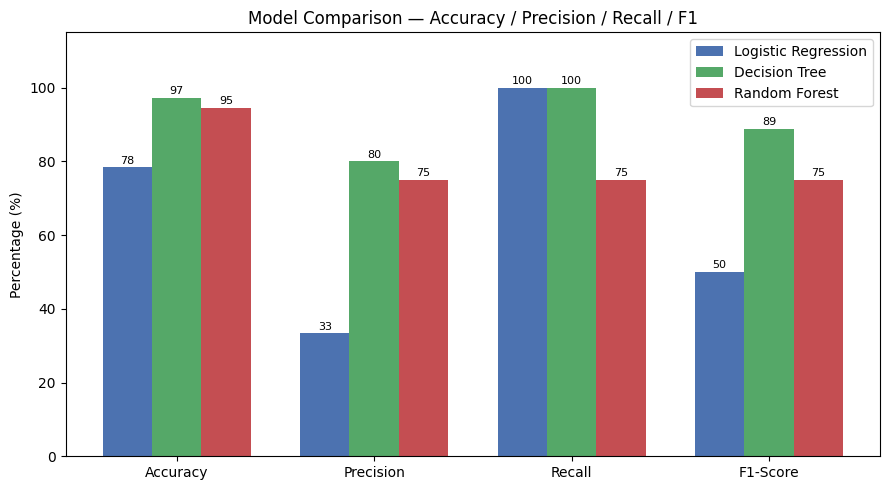
\includegraphics[width=0.95\columnwidth]{fig_comparison_metrics.png}
\caption{Per-metric comparison across the three classifiers.}
\label{fig:cmp-metrics}
\end{figure}

\begin{figure}[!t]
\centering
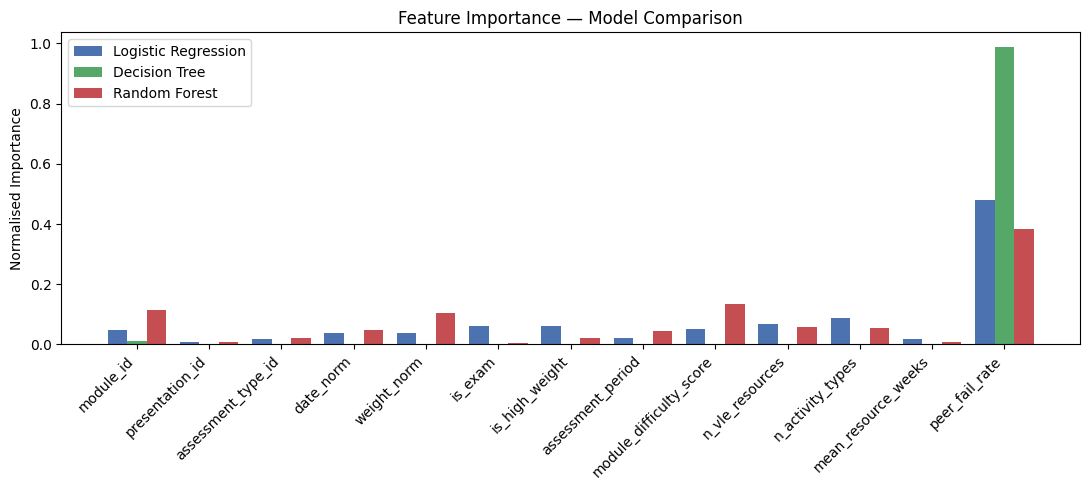
\includegraphics[width=0.95\columnwidth]{fig_comparison_feature_importance.png}
\caption{Normalised feature importance across LR (linear-weight magnitude), DT (Gini-gain), and RF (averaged Gini-gain). The leave-one-out \texttt{peer\_fail\_rate} dominates in every model.}
\label{fig:cmp-featimp}
\end{figure}

Two things stand out. The Decision Tree wins on three of the four metrics (Accuracy, Precision, F1) and ties Logistic Regression on Recall, which makes it the strongest single model to deploy. All three models also agree that \texttt{peer\_fail\_rate} is the most informative feature. They just back this up differently: LR puts a large positive weight on it ($+3.708$), the Decision Tree splits on it at the root, and the Random Forest concentrates most of its averaged Gini gain on it too. The models diverge in the tail. LR keeps meaningful weight on \texttt{n\_activity\_types} and the \texttt{is\_exam}/\texttt{is\_high\_weight} flags, the Decision Tree spreads the rest across \texttt{weight\_norm} and \texttt{n\_vle\_resources}, and the Random Forest distributes importance more evenly since its $50$ trees see different feature subsets. That all three algorithms land on the same top feature is a useful sanity check: the peer signal is a real predictor, not a quirk of any single method.

If Recall is the priority for an early-warning deployment, both LR and the Decision Tree work; we prefer the Decision Tree because it keeps perfect recall and cuts the false alarm rate dramatically. The Random Forest's lower recall makes it less suitable at this threshold, though it does illustrate the variance reduction from bagging. In production we would either ship the Decision Tree directly, or drop the Random Forest's threshold below $0.5$ to recover recall if an ensemble is preferred.

\section{Conclusion}
This study built an end-to-end pipeline that predicts High Risk assessments in OULAD. We derived the target from actual student outcomes rather than from the metadata columns used as features, which removed the target-leakage issue that gave a fake $100\%$ score in an earlier version. Thirteen features were engineered from three OULAD tables, and the leave-one-out peer fail-rate turned out to be the dominant predictor for every classifier we trained. We implemented three classifiers (Logistic Regression, Decision Tree, and Random Forest) from scratch in pure-stdlib Python and trained them with matched class-weighted objectives on the same stratified $80$/$20$ split. The Decision Tree was the strongest: $97.30\%$ accuracy, $80.00\%$ precision, $100.00\%$ recall, $88.89\%$ F1. Logistic Regression matched its recall but at lower precision. The Random Forest sat between them on accuracy and precision and lost one true positive on the small test set. All three models agreed on the importance of \texttt{peer\_fail\_rate}, which gives cross-model confidence in the engineered signal. For an OULAD-style early-warning use case where false negatives hurt much more than an extra flag, the Decision Tree is our recommended single-model choice.

\subsection{Future Scope}
A few extensions would push the pipeline further. Pivoting to student-level modelling (joined with \texttt{studentInfo.csv} and, where available, \texttt{studentVle.csv} click-streams) would support personalised risk scores and fairness checks across IMD band, region, and disability status. Temporal cross-validation across semesters would mimic real deployment more closely than random stratification, though the current $2013$/$2014$ snapshot is too thin for that at module level. Adding L$_2$ regularisation to gradient descent would help with overfitting on the small ($n=188$) dataset. Finally, loading the trained model into a star-schema warehouse with an assessment-keyed fact table would turn this into a live dashboard that refreshes as new \texttt{studentAssessment.csv} rows come in.

\begin{thebibliography}{99}
\bibitem[I]{ref1} C. Romero and S. Ventura, ``Educational data mining: A review of the state of the art,'' \textit{IEEE Transactions on Systems, Man, and Cybernetics, Part C}, vol. 40, no. 6, pp. 601--618, 2010.

\bibitem[II]{ref2} K. E. Arnold and M. D. Pistilli, ``Course Signals at Purdue: Using learning analytics to increase student success,'' in \textit{Proceedings of the 2nd International Conference on Learning Analytics and Knowledge (LAK)}, pp. 267--270, 2012.

\bibitem[III]{ref3} J. Kuzilek, M. Hlosta, and Z. Zdrahal, ``Open University Learning Analytics Dataset,'' \textit{Scientific Data}, vol. 4, no. 170171, 2017.

\bibitem[IV]{ref4} S. Chaudhuri and U. Dayal, ``An overview of data warehousing and OLAP technology,'' \textit{ACM SIGMOD Record}, vol. 26, no. 1, pp. 65--74, 1997.

\bibitem[V]{ref5} R. Kimball and M. Ross, \textit{The Data Warehouse Toolkit: The Definitive Guide to Dimensional Modeling}, 3rd ed. Wiley, 2013.

\bibitem[VI]{ref6} G. King and L. Zeng, ``Logistic regression in rare events data,'' \textit{Political Analysis}, vol. 9, no. 2, pp. 137--163, 2001.

\bibitem[VII]{ref7} D. Micci-Barreca, ``A preprocessing scheme for high-cardinality categorical attributes in classification and prediction problems,'' \textit{ACM SIGKDD Explorations}, vol. 3, no. 1, pp. 27--32, 2001.

\bibitem[VIII]{ref8} Y. Cui, M. Jia, T.-Y. Lin, Y. Song, and S. Belongie, ``Class-balanced loss based on effective number of samples,'' in \textit{Proceedings of the IEEE Conference on Computer Vision and Pattern Recognition (CVPR)}, pp. 9268--9277, 2019.

\bibitem[IX]{ref9} A. Hamoud, H. Adday, T. Obaid, and R. Hameed, ``Design and implementing cancer data warehouse to support clinical decisions,'' \textit{International Journal of Scientific \& Engineering Research}, vol. 7, no. 2, pp. 1271--1285, 2016.

\bibitem[X]{breiman2001rf} L. Breiman, ``Random Forests,'' \textit{Machine Learning}, vol. 45, no. 1, pp. 5--32, 2001.

\bibitem[XI]{cart1984} L. Breiman, J. H. Friedman, R. A. Olshen, and C. J. Stone, \textit{Classification and Regression Trees}. Wadsworth, 1984.
\end{thebibliography}

\end{document}
